%*----------- SLIDE -------------------------------------------------------------
\begin{frame}[t]{Introdução} 
    \transdissolve[duration=0.5]
    Título do projeto: Walker: um robô bípede

    Orientador: Marco A. dos Reis
    \newline
    \newline
    Sobre o orientador:
    %\newline
        \begin{columns}[t]
            \column{.05\linewidth}
            \column{1\linewidth}
                \begin{itemize}
                    \item Graduado em Engenharia Elétrica pela UFPR e Mestre em Engenharia de Produção pela UFSC
                    \item Pesquisador do Instituto Brasileiro de Robótica, uma ação conjunta entre o Senai Cimatec e o Centro Alemão de Inteligência Artificial
                    \item Professor convidado dos cursos de especialização em Automação, Controle e Robótica, e de Sistemas Elétricos de Potência do Senai CIMATEC
                \end{itemize}
            \column{.6\linewidth}
        \end{columns}
%*----------- notes
    \note[item]{Notes can help you to remember important information. Turn on the notes option.}
\end{frame}
%-
%*----------- SLIDE -------------------------------------------------------------
\begin{frame}[c]{Justificativa}
    %\cutpic{0.30cm}{3cm}{element}
    \begin{tabular}{cccc}
        \rule{73pt}{0ex}  &   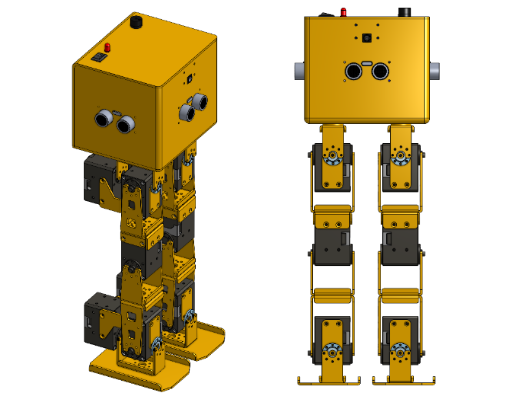
\includegraphics[width=.55\textwidth ]{walker.png}
    \end{tabular}

%*----------- notes
    \note[item]{Notes can help you to remember important information. Turn on the notes option.}
\end{frame}
%-
%*----------- SLIDE -------------------------------------------------------------
\begin{frame}[c]{Problema de pesquisa} 
    \transdissolve[duration=0.5]
   
    \begin{center}
        \Wider{%
        \begin{shaded}
        \begin{center}
            \vspace*{0.4cm}
            \resizebox{!}{1.3cm}{%
               % \color{bg} O objetivo é ter um objetivo.
                \begin{tabular}{ccc}
                    De que forma garantir a segurança humana em ambientes \\
                    confinados e de difícil acesso através da ajuda de \\ 
                    robôs bípedes?       
                  \end{tabular}
            }%
        \end{center}
        \end{shaded}
        }%
    \end{center}
    
   
%*----------- notes
    \note[item]{Notes can help you to remember important information. Turn on the notes option.}
\end{frame}
%-
%*----------- SLIDE -------------------------------------------------------------
\begin{frame}[t]{Objetivos} 
    \transdissolve[duration=0.5]
    
        Desenvolver um robô de pequeno porte que se desloca sobre dois pés. O robô deve ser capaz de se locomover e desviar de obstáculos em um determinado ambiente.
        \newline
        \newline
         Específicos:
        \begin{columns}[t]
            \column{.15\linewidth}
            \column{1\linewidth}
                \begin{enumerate}
                    \item Desenvolver algoritmos utilizando o ROS2
                    \item Implementar visão computacional para a navegação
                    \item Simular o sistema robótico
                    \item Implementar principais funcionalidades de um humanóide
                    \item Realizar demonstração do sistema
                    \item Desenvolver artigos científicos
                \end{enumerate}
            \column{.6\linewidth}
        \end{columns}
%*----------- notes
    \note[item]{Notes can help you to remember important information. Turn on the notes option.}
\end{frame}
%-
%*----------- SLIDE -------------------------------------------------------------
\begin{frame}[c]{Roadmap}
    %\cutpic{0.30cm}{3cm}{element}
    \begin{tabular}{cccc}
        \rule{30pt}{0ex}  &   
\includegraphics[width=.2\textwidth ]{element.png} & \rule{15pt}{0ex} 
\includegraphics[width=.15\textwidth]{notion.png} \rule{15pt}{0ex}& 
\includegraphics[width=.16\textwidth]{github.png}\\
    \end{tabular}

    \begin{tabular}{ccc}
        \phantom{The text is invisible} &   
\includegraphics[width=.2\textwidth]{trello.png} \rule{5pt}{0ex}& 
\includegraphics[width=.2\textwidth]{projectlibre.png} \\
    \end{tabular}
%*----------- notes
    \note[item]{Notes can help you to remember important information. Turn on the notes option.}
\end{frame}
%-
